\section{The WSN construction}
\begin{frame}{The WSN construction}
    \centering
    Published by \textcite{AC:Tessaro15} at AsiaCrypt 2015.
    \begin{columns}
        \begin{column}{0.49\textwidth}
            \begin{block}{Overview\vpPp}
                \centering
                \vspace*{13pt}
                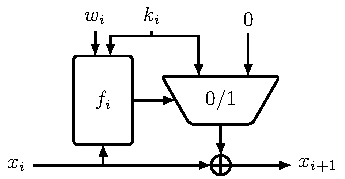
\includegraphics{data/wsn}
                \vspace*{13pt}
            \end{block}
        \end{column}
        \begin{column}{0.49\textwidth}
            \begin{block}{Whitened Swap-Or-Not round function}
                \vspace*{-10pt}
                \begin{equation*}
                    x_i \mapsto x_i + f_{b(i)}(w_i + \max \set{x_i, x_i + k_i}) \cdot k_i
                \end{equation*}
            \end{block}

            \begin{block}{Security Proposition (informal)}
                The WSN construction with $\mathcal{O}(n)$ rounds is
                \begin{equation*}
                    (2^{n-\mathcal{O}(\log n)}, 2^{n-\mathcal{O}(1)})\text{-secure}.
                \end{equation*}
            \end{block}
        \end{column}
    \end{columns}
    \blfootnote{$(p, q)$-secure: Attackers querying the encryption at most $p$ and the underlying $f_i$'s $q$ times have only negl.\ advantage.}
\end{frame}

\begin{frame}{Is this a practical alternative to AES?}{}
    \begin{columns}
        \begin{column}{0.49\textwidth}
            \begin{block}{An Implementation}
                \centering
                \vspace*{5pt}
                \visible<2->{%
                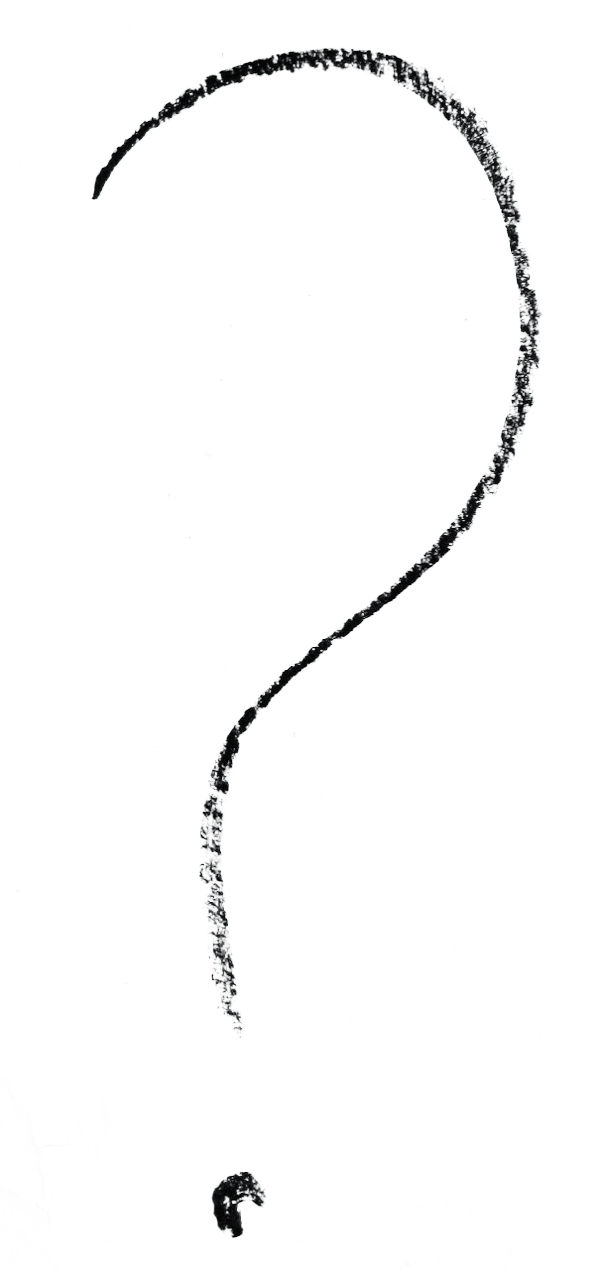
\includegraphics[height=35mm]{data/flickr/questionmark.png}
                }
                \vspace*{5pt}
            \end{block}
        \end{column}
        \begin{column}{0.49\textwidth}
            \visible<3->{%
            \begin{block}{Outline\vpPp}
                \setstretch{1.5}
                \vspace*{20pt}
                \hspace*{10pt}\begin{minipage}{0.75\textwidth}
                    \tableofcontents[sectionstyle=shaded/show]
                \end{minipage}
                \vspace*{12pt}
            \end{block}
            }
        \end{column}
    \end{columns}
\end{frame}

\section{Generic Analysis}
\begin{frame}{Generic Analysis}{On the number of rounds}
    \begin{columns}
        \begin{column}{0.49\textwidth}
            \begin{block}{Observation}
                \begin{itemize}
                    \item The ciphertext is the plaintext plus a random subset of the round keys:
                        \begin{equation*}
                            c = p + \sum_{i=1}^{r} \lambda_i k_i
                        \end{equation*}
                    \item For pairs $p_i, c_i$: $\Span \set{p_i + c_i} \subseteq \Span \set{k_j}$.
                \end{itemize}
            \end{block}
        \end{column}
        \begin{column}{0.49\textwidth}
            \begin{alertblock}{Problematic because}
                \vspace{1.5pt}
                \begin{itemize}
                    \item $\Span \set{k_j} \subset \F_2^n$ reveals one bit of information on the round keys\\[7pt]
                    \item for $r < n$ there exists probability one linear hulls,\\[7pt]
                    \item for $r < 2n - 3$ there exists zero correlation linear hulls.
                \end{itemize}
                \vspace{1.5pt}
            \end{alertblock}
        \end{column}
    \end{columns}
    \hspace*{-8.5pt}
    \begin{minipage}{1.0145\textwidth}
    \begin{exampleblock}{Rationale 1}
        Any instance must iterate at least n rounds; any set of n consecutive keys should be linear indp.
    \end{exampleblock}
    \end{minipage}
\end{frame}

\begin{frame}{Generic Analysis}{On the Boolean functions $f_i$}
    \begin{columns}
        \begin{column}{0.49\textwidth}
            \begin{block}{Observation}
                \begin{itemize}
                    \item If the $f_i$ do not depend on a (linear combination of) bit(s), \ie/
                        \begin{equation*}
                            f_i(x) = f_i(x + \delta)
                        \end{equation*}
                        this difference propagates through the whole encryption with non-negligible probability.
                \end{itemize}
            \end{block}
        \end{column}
        \begin{column}{0.49\textwidth}
            \begin{block}{}
            \end{block}
        \end{column}
    \end{columns}
    \hspace*{-8.5pt}
    \begin{minipage}{1.0145\textwidth}
    \begin{exampleblock}{Rationale 2}
        For any instance, the $f_i$ should depend on all bits, and for any $\delta \in \F_2^n:\ \Pr\bracket{f_i(x) = f_i(x + \delta)} \approx \frac{1}{2}$.
    \end{exampleblock}
    \end{minipage}
\end{frame}

\section{A first instance: \bison/}
\begin{frame}{The Instance}{Generic considerations}
    \begin{itemize}
        \item Use a bent function for $f_i$
        \item Use LFSRs for key schedule
    \end{itemize}
\end{frame}

\begin{frame}{The Instance}{\bison/'s round function}
    \begin{block}{BISON's round function}
        \centering
        \vspace{0.5\baselineskip}
        For round keys $k_i\in \F_2^n$ and $w_i\in \F_2^{n-1}$ the round function computes
        \begin{equation*}
            R_{k_i, w_i}(x) \coloneqq x + f_{b(i)} \parens{w_i + \Phi_{k_i}\parens{x}} \cdot k_i.
        \end{equation*}
        \flushleft
        where
        \begin{itemize}
            \item $\Phi_{k_i}$ is defined as in ???,
            \item $f_{b(i)}$ is defined as
                    \begin{align*}
                        f_{b(i)} : \F_2^{\frac{n-1}{2}}\times \F_2^{\frac{n-1}{2}} &\to \F_2 \\
                        f_{b(i)}(x,y) &\coloneqq \angles{x,y} + b(i),
                    \end{align*}
            \item and $b(i)$ is $0$ if $i \leqslant \frac{r}{2}$ and $1$ else.
        \end{itemize}
        \vspace{-0.25\baselineskip}
    \end{block}
\end{frame}

\begin{frame}{The Instance}{\bison/'s key schedule}
    \begin{block}{BISON's key schedule}
        \vspace{0.5\baselineskip}
        For two primitive polynomials $p_w(x),\, p_k(x) \in \F_2[x]$ with degrees $\deg(p_w) = n-1$ and $\deg(p_k) = n$ and the master key $K=(k,w) \in \F_2^n\times \F_2^{n-1}$, $k,w \ne 0$
        the key schedule computes the $i$th round keys as
        \begin{align*}
            \ks_i : \F_2^n \times \F_2^{n-1} &\to \F_2^n \times \F_2^{n-1} \\
            \ks_i(k, w) &\coloneqq (k_i, c_i + w_i)
        \end{align*}
        where $C(\cdot)$ is the companion matrix of the corresponding polynomial, and
        \begin{itemize}
            \item $k_i = {C(p_k)}^i k$
            \item $c_i = {C(p_w)}^{-i} e_1$
            \item $w_i = {C(p_w)}^i w$
        \end{itemize}
        \vspace{0.5\baselineskip}
    \end{block}
\end{frame}

\section{Differential Analysis}
\begin{frame}{Differential Cryptanalysis}{One round}
\end{frame}

\begin{frame}{Differential Cryptanalysis}{More rounds}
\end{frame}

\section{Further Analysis}
\begin{frame}{Further Cryptanalysis}
    \begin{itemize}
        \item Linear Cryptanalysis
        \item Impossible Differentials
        \item Zero Correlation
        \item Invariant Attacks
    \end{itemize}
\end{frame}

\begin{frame}{Conclusion/Questions}{Thank you for your attention!}
    \begin{columns}
        \begin{column}{0.5\textwidth}
            \begin{block}{\bison/}
                \begin{itemize}
                    \item A first instance of the WSN construction
                    \item Good results for differential cryptanalysis
                \end{itemize}
            \end{block}
            \begin{block}{Open Problems}
                \begin{itemize}
                    \item Construction with similar good results for linear cryptanalysis
                    \item Further analysis: division properties
                \end{itemize}
            \end{block}
        \end{column}
        \begin{column}{0.39\textwidth}
        \begin{figure}[!htb]
            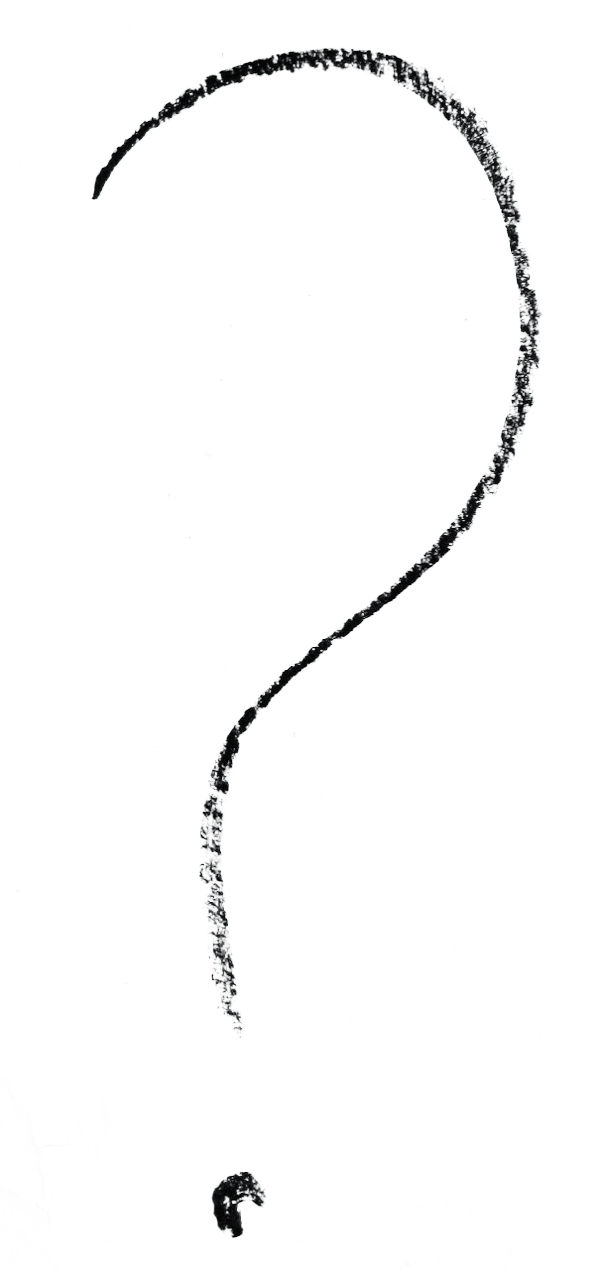
\includegraphics[height=50mm]{data/flickr/questionmark.png}
        \end{figure}
        \end{column}
    \end{columns}
    \blfootnote{\scriptsize Mainboard \& Questionmark Images: flickr}
\end{frame}

\begin{frame}[allowframebreaks]{References}
    \tiny
    \printbibliography{}
\end{frame}
